% witness: synthetic (the figure shape of 1104.5392, 1601.05000: `\includegraphics[width=\textwidth]` of a small PDF)
% oracle:  pdflatex 0 errors; the first and third figures \textwidth wide, the second at its natural 216x108 bp,
%          the fourth at half size
% engines: rust INT081TR = one quadrants.svg for all four, root 216x108 (the size of none but the natural one)
% expect:  0 errors, 0 warnings; HTML (EXT=html): x1.svg root width="476" height="238" (figures 1 and 3, one file),
%          quadrants.svg root as the converter wrote it (figure 2, byte-identical to INT081TR's quadrants.svg), x2.svg
%          root width="108" height="54" (figure 4); every viewBox "0 0 216 108"
% status:  RED (INT081TR) -> GREEN (SVGSCALE)
% preload: ar5iv.sty
\documentclass{article}
\usepackage{graphicx}
\begin{document}
\begin{figure}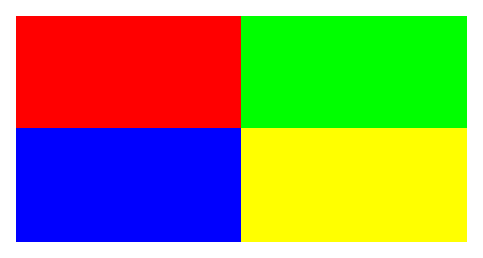
\includegraphics[width=\textwidth]{quadrants}\caption{Wide.}\end{figure}
\begin{figure}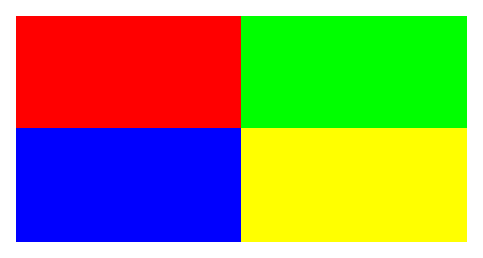
\includegraphics{quadrants}\caption{Natural.}\end{figure}
\begin{figure}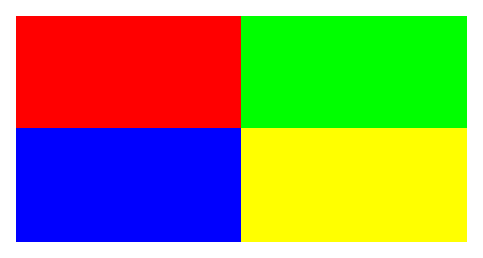
\includegraphics[width=\textwidth]{quadrants}\caption{Wide again.}\end{figure}
\begin{figure}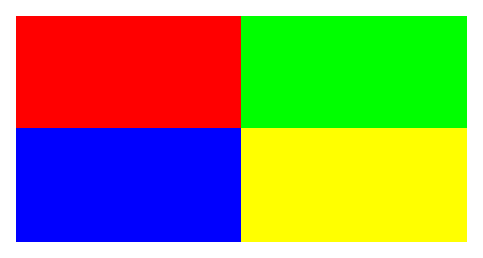
\includegraphics[scale=0.5]{quadrants}\caption{Half.}\end{figure}
\end{document}
